%%%%%%%%%%%%%%%%%%%%%%%%%%%%%%%%%%%
%This is the LaTeX ARTICLE template for RSC journals
%Copyright The Royal Society of Chemistry 2016
%%%%%%%%%%%%%%%%%%%%%%%%%%%%%%%%%%%

\documentclass[twoside,twocolumn,9pt]{article}
\usepackage{extsizes}
\usepackage[super,sort&compress,comma]{natbib} 
\usepackage[version=3]{mhchem}
\usepackage[left=1.5cm, right=1.5cm, top=1.785cm, bottom=2.0cm]{geometry}
\usepackage{balance}
\usepackage{times,mathptmx}
\usepackage{sectsty}
\usepackage{graphicx} 
\usepackage{lastpage}
\usepackage[format=plain,justification=justified,singlelinecheck=false,font={stretch=1.125,small,sf},labelfont=bf,labelsep=space]{caption}
\usepackage{float}
\usepackage{fancyhdr}
\usepackage{fnpos}
\usepackage[english]{babel}
\usepackage{array}
\usepackage{droidsans}
\usepackage{charter}
\usepackage[T1]{fontenc}
\usepackage[usenames,dvipsnames]{xcolor}
\usepackage{setspace}
\usepackage[compact]{titlesec}
%%%Please don't disable any packages in the preamble, as this may cause the template to display incorrectly.%%%


\usepackage{epstopdf}%This line makes .eps figures into .pdf - please comment out if not required.

\definecolor{cream}{RGB}{222,217,201}

\begin{document}

\pagestyle{fancy}
\thispagestyle{plain}
\fancypagestyle{plain}{

%%%HEADER%%%
\fancyhead[C]{
\includegraphics[width=18.5cm]{head_foot/header_bar}}
\fancyhead[L]{\hspace{0cm}\vspace{1.5cm}
\includegraphics[height=30pt]{head_foot/journal_name}}
\fancyhead[R]{\hspace{0cm}\vspace{1.7cm}
\includegraphics[height=55pt]{head_foot/RSC_LOGO_CMYK}}
\renewcommand{\headrulewidth}{0pt}
}
%%%END OF HEADER%%%

%%%PAGE SETUP - Please do not change any commands within this section%%%
\makeFNbottom
\makeatletter
\renewcommand\LARGE{\@setfontsize\LARGE{15pt}{17}}
\renewcommand\Large{\@setfontsize\Large{12pt}{14}}
\renewcommand\large{\@setfontsize\large{10pt}{12}}
\renewcommand\footnotesize{\@setfontsize\footnotesize{7pt}{10}}
\makeatother

\renewcommand{\thefootnote}{\fnsymbol{footnote}}
\renewcommand\footnoterule{\vspace*{1pt}% 
\color{cream}\hrule width 3.5in height 0.4pt \color{black}\vspace*{5pt}} 
\setcounter{secnumdepth}{5}

\makeatletter 
\renewcommand\@biblabel[1]{#1}            
\renewcommand\@makefntext[1]% 
{\noindent\makebox[0pt][r]{\@thefnmark\,}#1}
\makeatother 
\renewcommand{\figurename}{\small{Fig.}~}
\sectionfont{\sffamily\Large}
\subsectionfont{\normalsize}
\subsubsectionfont{\bf}
\setstretch{1.125} %In particular, please do not alter this line.
\setlength{\skip\footins}{0.8cm}
\setlength{\footnotesep}{0.25cm}
\setlength{\jot}{10pt}
\titlespacing*{\section}{0pt}{4pt}{4pt}
\titlespacing*{\subsection}{0pt}{15pt}{1pt}
%%%END OF PAGE SETUP%%%

%%%FOOTER%%%
\fancyfoot{}
\fancyfoot[LO,RE]{\vspace{-7.1pt}
\includegraphics[height=9pt]{head_foot/LF}}
\fancyfoot[CO]{\vspace{-7.1pt}\hspace{13.2cm}
\includegraphics{head_foot/RF}}
\fancyfoot[CE]{\vspace{-7.2pt}\hspace{-14.2cm}
\includegraphics{head_foot/RF}}
\fancyfoot[RO]{\footnotesize{\sffamily{1--\pageref{LastPage} ~\textbar  \hspace{2pt}\thepage}}}
\fancyfoot[LE]{\footnotesize{\sffamily{\thepage~\textbar\hspace{3.45cm} 1--\pageref{LastPage}}}}
\fancyhead{}
\renewcommand{\headrulewidth}{0pt} 
\renewcommand{\footrulewidth}{0pt}
\setlength{\arrayrulewidth}{1pt}
\setlength{\columnsep}{6.5mm}
\setlength\bibsep{1pt}
%%%END OF FOOTER%%%

%%%FIGURE SETUP - please do not change any commands within this section%%%
\makeatletter 
\newlength{\figrulesep} 
\setlength{\figrulesep}{0.5\textfloatsep} 

\newcommand{\topfigrule}{\vspace*{-1pt}% 
\noindent{\color{cream}\rule[-\figrulesep]{\columnwidth}{1.5pt}} }

\newcommand{\botfigrule}{\vspace*{-2pt}% 
\noindent{\color{cream}\rule[\figrulesep]{\columnwidth}{1.5pt}} }

\newcommand{\dblfigrule}{\vspace*{-1pt}% 
\noindent{\color{cream}\rule[-\figrulesep]{\textwidth}{1.5pt}} }

\makeatother
%%%END OF FIGURE SETUP%%%

%%%TITLE, AUTHORS AND ABSTRACT%%%
\twocolumn[
  \begin{@twocolumnfalse}
\vspace{3cm}
\sffamily
\begin{tabular}{m{4.5cm} p{13.5cm} }


\includegraphics{head_foot/DOI} & \noindent\LARGE{\textbf{A Method for Studying the Diffusion of Quaternary Ammonium Cations Through Polyelectrolyte Phases$^\dag$}} \\%Article title goes here instead of the text "This is the title"
\vspace{0.3cm} & \vspace{0.3cm} \\

 & \noindent\large{Alexander M. Papiez,$^{\ast}$\textit{$^{a}$} Justin J. B. Perry,\textit{$^{b\ddag}$} and Les R. Dix\textit{$^{a}$}} \\%Author names go here instead of "Full name", etc.


\includegraphics{head_foot/dates} & \noindent\normalsize{The mobility of organic cations in polymeric phases is an important property to consider when using these materials as active ingredients in coatings. Here we describe a method for extracting such compounds from polymeric samples and how analysis of these extracts can yield insights about the diffusivity of molecules in a polymeric phase.} \\%The abstrast goes here instead of the text "The abstract should be..."

\end{tabular}

 \end{@twocolumnfalse} \vspace{0.6cm}

  ]
%%%END OF TITLE, AUTHORS AND ABSTRACT%%%

%%%FONT SETUP - please do not change any commands within this section
\renewcommand*\rmdefault{bch}\normalfont\upshape
\rmfamily
\section*{}
\vspace{-1cm}


%%%FOOTNOTES%%%

\footnotetext{\textit{$^{a}$~Address, Address, Town, Country. Fax: XX XXXX XXXX; Tel: XX XXXX XXXX; E-mail: xxxx@aaa.bbb.ccc}}
\footnotetext{\textit{$^{b}$~Address, Address, Town, Country. }}

%Please use \dag to cite the ESI in the main text of the article.
%If you article does not have ESI please remove the the \dag symbol from the title and the footnotetext below.
\footnotetext{\dag~Electronic Supplementary Information (ESI) available: [details of any supplementary information available should be included here]. See DOI: 10.1039/b000000x/}
%additional addresses can be cited as above using the lower-case letters, c, d, e... If all authors are from the same address, no letter is required

\footnotetext{\ddag~Additional footnotes to the title and authors can be included \textit{e.g.}\ `Present address:' or `These authors contributed equally to this work' as above using the symbols: \ddag, \textsection, and \P. Please place the appropriate symbol next to the author's name and include a \texttt{\textbackslash footnotetext} entry in the the correct place in the list.}


%%%END OF FOOTNOTES%%%

%%%MAIN TEXT%%%%
%\subsection{This is the subsection heading style}
%Section headings can be typeset with and without numbers.\cite{Abernethy2003}

%\subsubsection{This is the subsubsection style.~~} These headings should end in a full point.  

%\paragraph{This is the next level heading.~~} For this level please use \texttt{\textbackslash paragraph}. These headings should also end in a full point.

\section{Introduction}
Diffusion in polymeric phases is an important phenomenon which influences many fields. The ability to control the release of active compounds from a polymeric vehicle may be influenced by the diffusivity of these compounds, especially when strong interactions exist between the active compound and the vehicle. Particularly interesting are those cases in which these interactions can be modified to tune the diffusivity of the mobile compound. 

In order to assess how different structural features assess the diffusivity of an analyte, the kinetics of analyte release must be measured. The methods used to effect this measurement are highly dependant on both the nature and quantity of the analyte of interest. 

\begin{table}[h]
\small
  \caption{\ Some typical methods used to detect different types of analyte}
  \label{tbl:example}
  \begin{tabular*}{0.48\textwidth}{@{\extracolsep{\fill}}lll}
    \hline
    Analyte & Detection Method & Sensitivity \\
    \hline
    Transition metal & Flame Photometry & 10-1000 ppm\\
                     & Flame AAS        & 1-100 ppm\\
                     & Flame AES        & < 1 ppm \\
    Organic Cations  & HPLC-MS          & 10ppb - 10 ppm\\
                     & GC-MS            & 10ppb - 10 ppm\\
                     & qNMR             & 10 - 1000 ppm\\
                     \hline
  \end{tabular*}
\end{table}

While HPLC-MS and GC-MS are by far the most sensitive techniques for the investigation of organic compounds, much time and effort must be spent developing and optimizing analyte extraction, pre-concentration and detection methods. Alternative methods, such as flame-photometry and quantitative NMR spectroscopy require less method development but are concomitantly less sensitive. The aim of this work was to establish whether the kinetics of the ion exchange of quaternary ammonium cations could be studied using a combination of flame photometry and qNMR.

\section{Ion Exchange}
\begin{figure}[h !]
	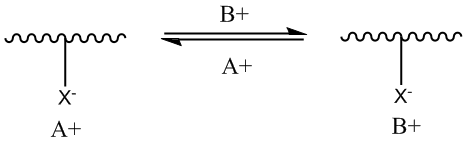
\includegraphics[width=.5\textwidth]{images/ion_exchange}
	\caption{Basic outline of the ion exchange equilibrium, where an incoming ion B+ can displace a resin associated ion A+ }
	\label{fig:ion_ex}
\end{figure}

\subsection{Basic Principle}
Ion exchange describes the phenomenon in which an ion exchange material in some initial ionic form will, in contact with a solution containing some ion of a different type to that already contained within the resin, will take-up that ion while releasing the initial ion. 

\begin{equation}
R\bar{A} + B^+ \leftrightarrow R\bar{B} + A^+
\end{equation}

This phenomenon is of great utility in a large number of industrially important processes; notably the preferential extraction of radioactive isotopes from the waste produced by nuclear reactors.

\subsection{Ion Exchange materials}
A typical ion exchange material consists of a crosslinked polymeric matrix containing acidic or basic side chains (depending upon whether cation or anion exchange is the desired behaviour of the resin). One of the most popular co-polymers used as a matrix for ion-exchange material is styrene-divinylbenzene (SDVB)(see figure \ref{fig:sdvb}).

\begin{figure}[h !]
	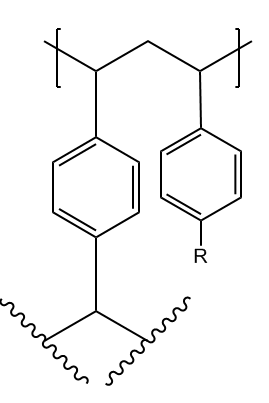
\includegraphics[height=.2\textheight]{images/sdvb}
	\centering
	\caption{The styrene-divinylbenzene co-polymer is one of the most popular skeletons for ion exchange resins. R may be any acidic or basic group, dependant upon whether cation or anion exchange functionality is desired}
	\label{fig:sdvb}
\end{figure}

SDVB based resins are particularly attractive due to the ease with which polymer beads of a well controlled size distribution may be obtained. This is achieved by inverse phase suspension free radical polymerization of the monomers in water.  As we shall later discuss, this size control is critical for the production of ion exchange resins which behave in a well defined and predictable manner.

\section{The Kinetics of Ion Exchange}
The kinetics of ion exchange are well understood, with the first pioneering studies undertaken by Hellferich at the beginning of the 20th century.\cite{helfferich1962} The early consensus which was established is that diffusion of ions is the rate-controlling step in ion exchange reactions. There are however two separate diffusive mechanisms which may dominate, depending on reaction conditions, the structure of the ion exchange resin and the nature of the ions undergoing exchange.

\begin{figure}[h !]
	\centering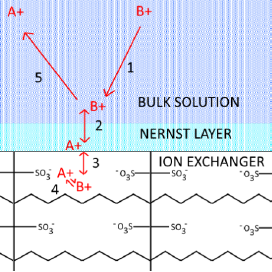
\includegraphics[height=.3\textwidth]{images/types_of_diffusion}
	\caption{Ion exchange consists of a number of steps; 1+5: diffusion of ions through the bulk solution, 2: diffusion of ions through the Nernst Layer, 3: diffusion of ions through the polymeric phase, 4: exchange of ions at the ionic polymer side chain}
	\label{fig:diftypes}
\end{figure}
\section{Equations}

Figure \ref{fig:diftypes} shows the various sub-processes which make up the overall ion exchange process. It is widely accepted that of all these processes, only diffusion through the Nernst layer and the ion exchanger itself are rate controlling (processes 2 and 3 respectively).\cite{helfferich1962} 

When studying the ion exchange reaction it is important to determine which diffusion type is rate controlling; not only are they subject to significantly different mathematical interpretations, they shed light on diffusion in different regions. In other words, to study diffusivity of a molecule within a polymeric phase, particle diffusion not film diffusion must be rate controlling. Table \ref{tab:diff_type_control} shows how the reaction conditions can be modified in order to influence which process will be rate controlling. 

\begin{table}[h]
	\small
	\caption{The effect of different reaction conditions on the two potential rate controlling diffusion types}
	\label{tbl:example}
	\begin{tabular*}{0.48\textwidth}{@{\extracolsep{\fill}}lll}
		\hline
		Condition & Particle Diffusion & Film Diffusion\\
		          &                    & Control \\
		\hline
		Ion mobility in particle & $\propto$ mobility & No effect\\
		In bulk solution& No effect   & $\propto$ mobility \\
		Particle size& $\frac{1}{r^2}$  & $\propto \frac{1}{r}$ \\
		Capacity of exchanger  &  no effect   & $\propto \frac{1}{X}$\\
		Nature of ionic groups & $\propto$ strength of &  No effect\\
		                       &  electrostatic interaction & \\
		Degree of cross-linking & $\propto \frac{1}{crosslink degree}$  & No effect\\
		\hline
	\end{tabular*}
	\label{tab:diff_type_control}
\end{table}

 \[ A = \pi r^2 \]

\begin{equation}
  \frac{\gamma}{\epsilon x} r^2 = 2r
\end{equation}

You can also put lists into the text. You can have bulleted or numbered lists of almost any kind. 
The \texttt{mhchem} package can also be used so that formulae are easy to input: \texttt{\textbackslash ce\{H2SO4\}} gives \ce{H2SO4}. 

For footnotes in the main text of the article please number the footnotes to avoid duplicate symbols. \textit{e.g.}\ \texttt{\textbackslash footnote[num]\{your text\}}. The corresponding author $\ast$ counts as footnote 1, ESI as footnote 2, \textit{e.g.}\ if there is no ESI, please start at [num]=[2], if ESI is cited in the title please start at [num]=[3] \textit{etc.} Please also cite the ESI within the main body of the text using \dag.

\section{Conclusions}
The conclusions section should come at the end of article. For the reference section, the style file \texttt{rsc.bst} can be used to generate the correct reference style.
%%%END OF MAIN TEXT%%%

%The \balance command can be used to balance the columns on the final page if desired. It should be placed anywhere within the first column of the last page.

\balance

%If notes are included in your references you can change the title from 'References' to 'Notes and references' using the following command:
%\renewcommand\refname{Notes and references}

%%%REFERENCES%%%
\bibliography{rsc} %You need to replace "rsc" on this line with the name of your .bib file
\bibliographystyle{rsc} %the RSC's .bst file

\end{document}
